\subsection{Preparation}
After the initial alignment mentioned by \cite{deny_hamel} up to step 6, in order to see interference fringes one must pre-align the interferometer. This is done by first removing the half-wave plate (HWP)
from the inside of the interferometer.\\
Next, it is importanat to place two irises, one just after the output of the main PBS, and the second one as far away from that one as room on the table will allow.
The reason for this is error propagation. It is much easier to see if the beams are misaligned over a larger distance.\\
Prepare a camera with its lens removed and make sure you can connect and see an image on your computer.\\
Place the camera on the table next to the iris closest to the PBS, make sure the iris is fully open (and the camera pointing the right direction ;) ),
and observe what happens when you change the beams' polarization using a HWP, going from H, to D, to V, and back. If the Sagnac Interferometer (SI) is badly misaligned,
you should be able to see two beams, spatially separated, when rotating the HWP. You may repeat this step for the second iris if you so wish.\\
\subsection{The fun part}
Start with the farthest iris and set the polarization of the pump to either H or V. Here you have to choose which mirrors will be your H mirrors, and which will be your V mirrors.
This is crutial for this to be a time efficient endeavor. It is an arbitrary choice, but one that needs to be made and respected throughout the enterity of the alignment process.
Choose them in an intuitive way for you. Based on \ref{fig:SI}, we choose the H mirrors to be C, and M2, and the V mirrors to be M0, and M1.

\begin{figure}[H]
\begin{center}
	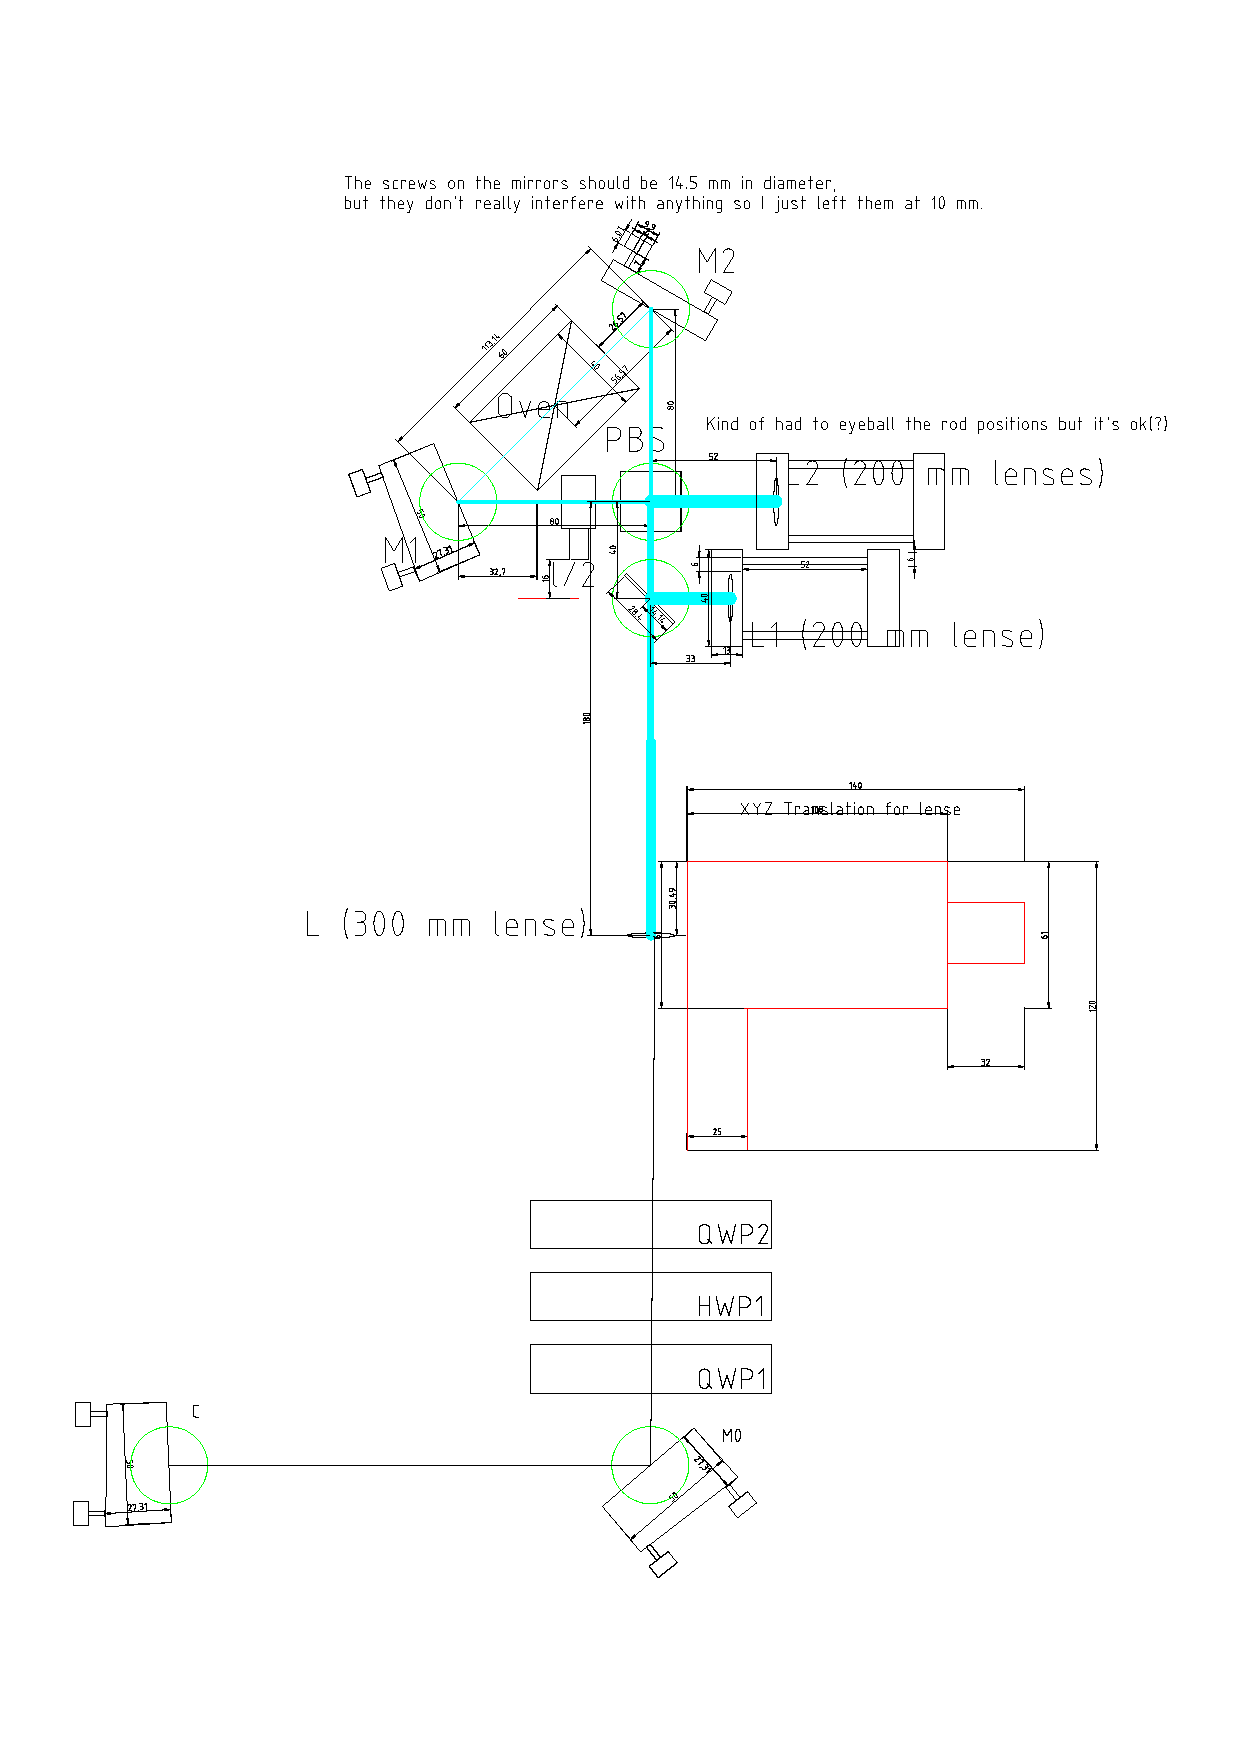
\includegraphics[scale=0.4]{Sagnac_Larger_300mm_Lens.pdf}
\end{center}
\caption{Our SI design}
\label{fig:SI}
\end{figure}

Once you have chosen which mirror (or coupler) you will use for alignment of a specific branch you can start the alignment.
The alignment is done in multiple steps for each branch. First, with the webcam, check again the positions of the H and V beams. You want them to be superimposed when you go to D. 
Lets say you start with H. The beam should go through the interferometer on the image \ref{fig:SI} from C $\rightarrow$ M0 $\rightarrow$ M2 $\rightarrow$ M1 and 
continue straight to the top lens for instance. The order of the last two mirrors will be switched for the other polarization. 
You place the webcam at the farthest iris and rotate the knobs on your H mirrors/coupler such that it moves through the center of the closed iris.
You want to move the farthest mirror (coupler) M0 (C) as little as possible as this will make the largest impact on the beampath.
Once you're sure the beam is going through the (almost) fully closed iris' center you move to the other branch.
Place the camera to the closer iris to the PBS. Change polarization on HWP1 to V. Do the same thing as described above until the beam passes through the center of the (almost) fully closed iris.
Next comes the important bit. Stay on V and move to the other iris. Now you will only move the horizontal knob in the V branch of the interferometer.
Repeat the above step to get the beam through the closed iris. Then do the same thing on the H branch at the farther away iris.
Repeat all of these steps until you see the two beams overlapping as much as possible. You will use this same method later as well when
optimizing the interference.
\begin{figure}[H]
\begin{center}
	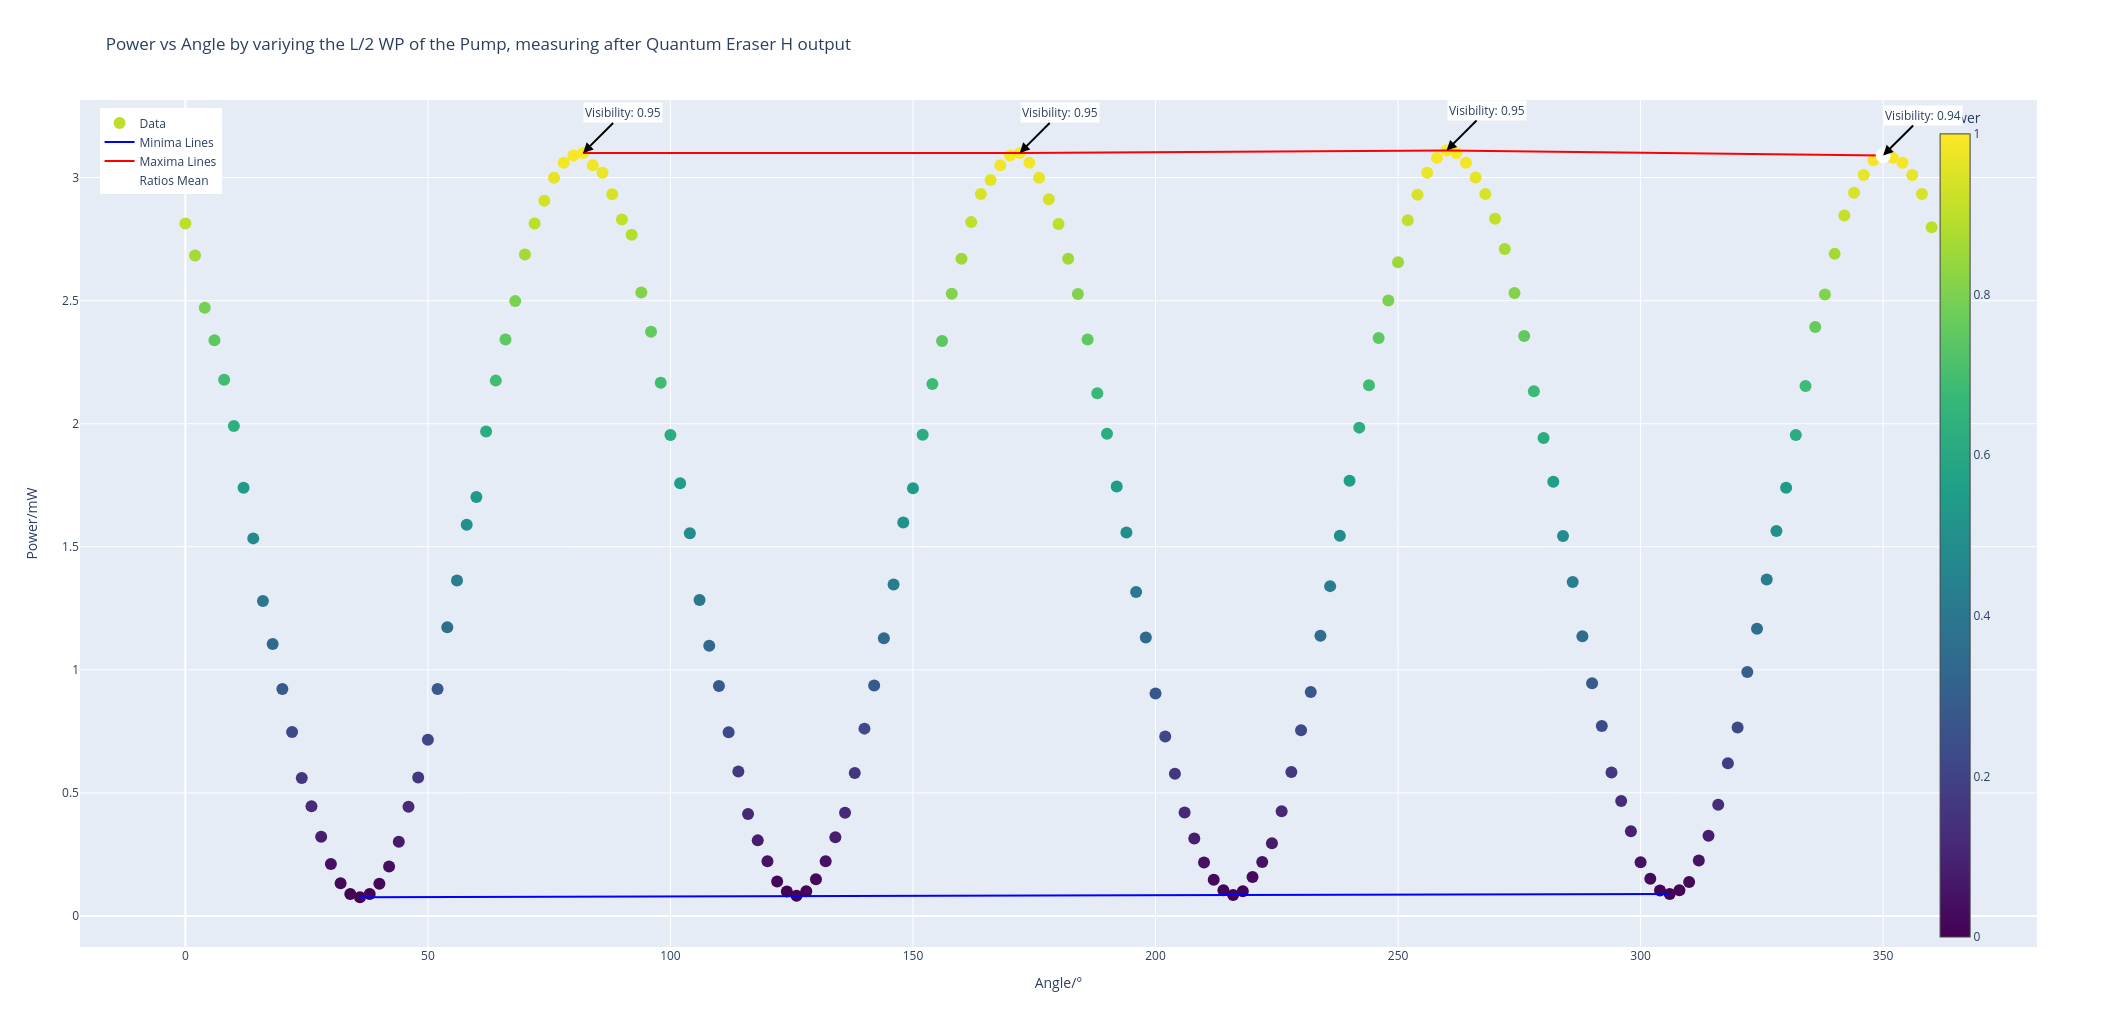
\includegraphics[width=12cm]{InterferencePlot.png}
\end{center}
\caption{Plotting the power of the transmitted beam after a quantum eraser. In image \ref{fig:SI} we have a part of the quantum eraser setup.
At the output of the PBS we have another HWP and PBS through which we measure the interference.}
\label{fig:InterferencePlot}
\end{figure}
